\section{Git operations}

\subsection{Add}

The add operation will just update the content of a file in the index, 
or add a new file to it, so in the next commit it can be commited. \par
When we are just updating the content of a file, Git also removes the file
with the old content.

\begin{lstlisting}
pred add[s,s' : State, f : File] {
	
	head.s' = head.s
	branches.s' = branches.s
	marks.s' = marks.s
	objects.s' = object.s

	index.s' = index.s + f .((f.path).~path -f)
}
\end{lstlisting}

\begin{figure}[h!] 
	\caption{Before the add}
	\centering
	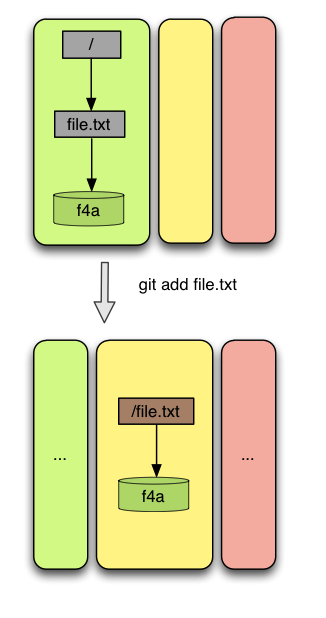
\includegraphics[scale=0.65]{images/add1.png}
\end{figure}

\begin{figure}[h!] 
	\caption{After the add}
	\centering
	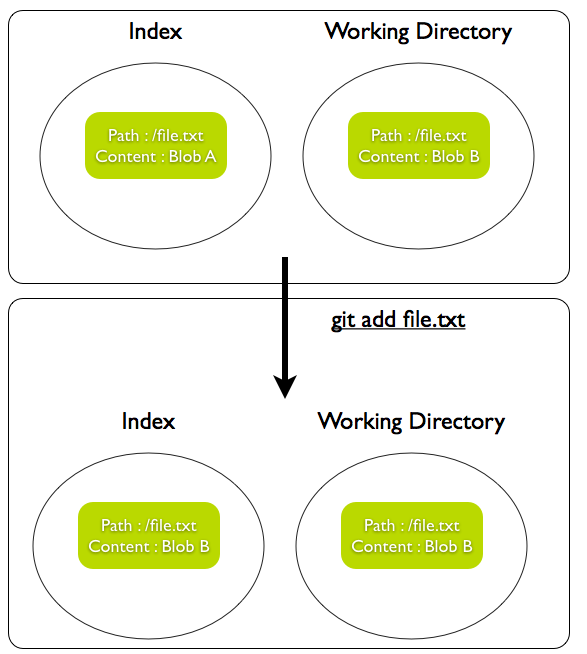
\includegraphics[scale=0.65]{images/add2.png}
\end{figure}

\pagebreak

\subsection{Remove}

Accordingly to man git-rm, removes files from the index, or from the
working tree and the index, so in the next commit it can be commited
it's removal. The file must exist in the
previous commit.\par

\begin{lstlisting}
pred remove[s,s' : State, f:File] {
	f in index.s
	f.path -> f.blob in (head.s).(marks.s).abs

	head.s' = head.s
	branches.s' = branches.s
	marks.s' = marks.s 
	objects.s' = objects.s
	index.s' = index.s - f
}
\end{lstlisting}

We can see the remove operation as the inverse of add, thus the rm 
operation can be represented as the figures 3 and 4 but in a inverse
order. \par

\subsection{Commit}

Accordingly to man git-commit, the commit operation 
stores the current contents of the index in a new commit 
along with a log message from the user describing the changes. \par 


\subsection{Branch}

Git branch operation has several forms, that to different things on git.
The ones wich we care are the forms that create a delete branches. \par
When a new branch is created it will point to the current HEAD by default.
\par
The man git-branch says that when deleting a branch, it must be fully
merged in its upstream branch, or in HEAD if no upstream was set. \par

\subsection{Checkout}

From man git-checkout : "Switches branches by updating the index, 
working tree, and HEAD to reflect the specified branch or commit". \par

\subsection{Merge}

From man git-merge : "Join two or mode development histories together" \par


